% Last Update Time-stamp: <04-03-2019>
\documentclass[12pt,twoside]{report}

\usepackage[utf8]{inputenc}
\usepackage[a4paper,margin=20mm,bindingoffset=10mm]{geometry}
\usepackage{graphicx}
\usepackage{booktabs}
\usepackage{refstyle}
\usepackage{caption}
\usepackage{titlesec}
\usepackage{fancyhdr}
\usepackage{color}
\usepackage{inconsolata}
\usepackage{listings}
\usepackage[UKenglish]{datetime}
\usepackage{pgf-umlsd}
\usepackage[T1]{fontenc}


\graphicspath{{images/}}

\title{Minimising Lag in Game Networking Models Without a Central Server}
\author{Szymon Jackiewicz}

\makeatletter
\let\thisauthor\@author
\let\thistitle\@title

\definecolor{pblue}{rgb}{0.13,0.13,1}
\definecolor{pgreen}{rgb}{0,0.5,0}
\definecolor{pred}{rgb}{0.9,0,0}
\definecolor{pgrey}{rgb}{0.46,0.45,0.48}
\lstset{language=C++,
  showspaces=false,
  showtabs=false,
  breaklines=true,
  showstringspaces=false,
  breakatwhitespace=true,
  commentstyle=\color{pgreen},
  keywordstyle=\color{pblue},
  stringstyle=\color{pred},
  basicstyle=\ttfamily,
  moredelim=[il][\textcolor{pgrey}]{$$},
  moredelim=[is][\textcolor{pgrey}]{\%\%}{\%\%}
}

\pagestyle{fancy}
\fancyhead{}
\fancyhead[L]{Game Networking Models}
\fancyhead[R]{\thisauthor}
\fancyfoot{}
\fancyfoot[C]{\thepage}

% Thesis format that corresponds to the Newcastle University standards
\titleformat{\chapter}[hang]{\normalfont\huge\bfseries}{\chaptertitlename\ \thechapter:}{1em}{}
\titleformat*{\section}{\normalfont\normalsize\bfseries}
\titleformat*{\subsection}{\normalfont\normalsize\bfseries}
\titleformat*{\subsubsection}{\normalfont\normalsize\bfseries}
\titlespacing*{\chapter}{0pt}{10pt}{30pt}

% The date should be in the UK Style DD MM YYYY
\newdateformat{UKvardate}{
  \THEDAY\ \monthname[\THEMONTH]\ \THEYEAR
}
\UKvardate

\begin{document}

\begin{titlepage}
  \begin{center}
    \makeatletter
    \vspace*{1cm}
    \Huge
    \textbf{\@title}\\
    \vspace*{0.5cm}
    \large
    Implementation and Analysis of Client-Hosted and Peer-to-Peer Networking Models in the Context of Games.\\


    \vspace*{2cm}
    \Large
    \textbf{\@author}\\
    \large
    Student Number: 150249751\\
    Supervisor: Dr Graham Morgan\\

    \vspace*{2cm}
    Word Count: 15,335\\

    \vfill

    
\includegraphics[width=0.4\textwidth]{Newcastle_University_logo.png}

    \Large
    MComp Computer Science w Games Engineering\\
    Stage 3\\
    \vspace*{1cm}
    Department of Computer Science\\
    Newcastle University\\
    \today
    \makeatother
  \end{center}
\end{titlepage}


\thispagestyle{plain}
\begin{center}
  \textbf{Declaration}
\end{center}

"I declare that this dissertation represents my own work except, where otherwise stated."

\newpage

\thispagestyle{plain}
\begin{center}
  \textbf{Acknowledgements}
\end{center}
I would like to thank this project's supervisor Dr. Graham Morgan, for the help and advice that he has provided throught all statges of this project. His guidance proved to be invaluable. I would also like to thank Laheem Khan for general help.

\newpage

\thispagestyle{plain}
\begin{center}
  \makeatletter
  \Large
  \textbf{\@title}

  \vspace*{0.4cm}
  \large
  Implementation and Analysis of Client-Hosted and Peer-to-Peer Networking Models in the Context of Games

  \vspace*{0.4cm}
  \textbf{\@author}

  \vspace*{0.9cm}
  \textbf{Abstract}
  \makeatother
\end{center}
A significant share of today's network traffic, consists of game networking. This is due to the emence amount of data that has to fundamentally be sent from client to client (or server) in order to keep a simulation synchronised between several participants. The fundamental principles of this mean that each client should be able to make a change (e.g. movement of their game character), and each other client that participates in the same instance of the simulation should be able to see this change on their local machine. There are several ways of achieving this.

The most common way of achieve a simulation that is synchronised across several users, is to introduce a trusted 3rd party entity that would essentially determine the ``Real'' state of the simulation. Each client participating in this instance, would submit their changes to this entity which would only implement the changes after checking for validity. The ``Real'' state would then be sent over to each client so that everyone can update their local simulations to it. Introducing a central entity like this provides a lot of advantages for everyone and is typically implemented by providing central servers that act as the 3rd party entity. The main advantages to this solution include fairness in latency and lag between all players and cheating prevention as all actions are approved before being accepted.

While this solution provides a lot of benefits to the playerbase of a game, it may not always be the best solution. The biggest problem that exists with this solution, is the cost that is associated with the deployment of these servers. Firstly, the cost of renting/running servers that are capable of handling the expected traffic and processing many instances of simulations at the same time could be very high. What makes this issue worse, is that if not enough of these servers are deployed, the experience of all players is compromised through large differences in player ping. This means that servers have to be deployed worldwide which involves further cost.

This downside can be overcome through avoiding the need for a central server through connecting to the other players directly, which introduces several compromises. The different ways of acomplishing a synchronised simulation, without a 3rd party entity, is what I will be investigating in this project through the implementation of 2 different ways of doing this; the Peer-to-Peer Model and the Client-Hosted model. I will be investigating the effectiveness of each solution across several scenarios and aim to come up with a guideline of which one should be used in given situations.


\tableofcontents

\chapter{Introduction}
Throughout this project, I will be exploring the different methods of providing a synchronised, multiplayer gaming experience on two or more computers on a network. I will be covering the networking basics of how two game clients running on seperate machines can communicate with each other as well as exploring the relevant details of how and why the networking systems in games are designed the way they are.


I will explore the existing methods of writing an online multiplayer game from scratch and aim to provide an implementation of a networking library for online games to communicate without a central server. I also aim to provide analysis of efficieny of different methods of achieving this goal.

\section{Project Goals}
When developing a multiplayer game the most important aspect of the codebase is likely to be the networking functionality and speed. In most games designed for two or more players interacting with each other or the environment, the whole experience can be ruined by slow or inefficient networking implementation. The most common way for games publishers/developers to address this, is to rent out servers space optimised for fast network speeds and a large amount of processing power. This allows each player to connect to a central known entity that can be trusted to be fast enough to handle the load of processing each simulation step and broadcasting information quickly. This solution provides many benefits in terms of security, cheating prevention and fairness, however it is an expensive investment and risk for games developed on a smaller budget.

I will be investigating other options that exist for the smaller budget projects and how to make the gameplay as seamless as possible with the limitations of consumer hardware and network connections. While some aspects of this, such as high ping between clients due to a bad network connection or suboptimal routing are out of control of the implementation, there are many ways that the game netcode can be implemented to minimise latency and provide a synchronised experience for all clients.
\\
\\
Implementation goals:
\begin{itemize}
\item Implement a system that allows one client to act as a server for all others. Throughout this document, I will be refering to this as the \textbf{Client-Hosted} model.
\item Implement a system for each client to send their updates to each other client directly. Throughout this document, I will be refering to this as the \textbf{Peer-to-Peer} model.
\end{itemize}
Data gathering goals:
\begin{itemize}
\item TODO
\end{itemize}

\newpage

\section{Basic concepts and terminolory}
First of all, I will define some basic concepts and terminolory that will be used throughout this document.
\\
\\
\textbf{Client}: Within the context of this document, a client can be defined as a piece of software responsible to running the game (i.e. game client). A client can also be defined as a computer interacting with a server, however it is possible to run two different instances of a game client on a single machine.
\\
\\
\textbf{Online Multiplayer Game}: A video game can be defined as a simulation of a certain scenario that can be manipulated by the player of the game. When talking about online multiplayer games, it can be thought of as a simulation that runs on several clients connected by a network (e.g. LAN or the Internet) that is to be synchronised. When one player performs an action that effects the state of the simulation, this action should also be seen by all participants of this perticular simulation instance and therefore the simulation should remain in the same state across all participating clients.
\\
\\
\textbf{Ping}: In network connections, the ping between different clients refers to the shortest amount of time that is needed for one client to send information to another and receive a response from this client. One client sends a ``ICMP echo request'' to another networked client (e.g. a game server). The receiving client, then responds with an ``ICMP echo reply'' back to the original device. The time between sending the request and receiving the reply, is the ping between the two clients.
\\
\\
\textbf{Lag}: The grater the ping between two connected clients, the bigger the difference in the state of each clients' simulation once an action to be synchronised is performed. When a change is made by one client, this change should be seen by other clients participating in the same simulation and lag occurs when this change does not appear instentaneous to the user.
\\
\\
\textbf{Jitter}: The difference in frequency that the messages are sent from a sender and received by the receiver. If a sending client sends packets at a constant rate, they would ideally arrive at the receiver's client at the same rate. This is not always the case however and could lead to some unwanted results in certain applications such as VOIP.


\newpage
\section{Networking principles in games}
TODO: talk a bit about UDP, TCP/IP and routing...

\subsection{Communitaction Issues}

In the dissertation \mycite{macedonia1995network}, the author has identified and grouped the most prevelent issues that occur in internet communications. In real time applications such as online games, these issues can be very impactful on the experience of the players.

\subsubsection{Data Distribution}
Broadcast to each client

\subsubsection{Latency}
Lag and Jitter


\subsubsection{Reliability}
UPD can lose packets........ The article \mycite{lincroft1999internet} documents the issues that the developement team encountered when developing the netcode for the 1997 game ``X-Wing vs. TIE fighter''. The author has experimented with TCP connections in game data transmission and found that ``TCP refuses to deliver any of the other packets in the stream while it waits for the next "in order" packet. This is why we would see latencies in the 5-second range.'' and ``if a packet is having a tough time getting to its destination, TCP will actually stop re-sending it! The theory is that if packets are being dropped that it's due to congestion.''. The features that have been implemented into TCP to make it reliable, end up negatively effecting real-time application data traffic and due to the volume of data to be transmitted, should not be used for time sensitive data.

\subsubsection{Bandwidth}
Consumer hardware and networking slow (esp upload)

\subsection{Inconsistant ping between players}
There are many different possible reasons for the lag to the server to vary widely from player to player. Firstly, it is possible that there are not enough servers throughout the world or that they are not spread out evenly enough across all regions. Players who live in geographically more remote locations, are likely to experience higher ping to servers compared to those that live in more densly populated cities due to where the servers are likely to be located. Secondly, there is no way of guaranteeing if the clients are going to be using a wired or a wireless connection to connect to the server. Wireless connections can be much slower and are more likely to introduce other potential problems such as packet loss.

Varying ping between players could lead to a problem of a poor experience for a client with a high ping to the server, as they will receive the updates from the server later than every other player and therefore be at a disadvantage if the game requires real time reactions. Unfortunately under some implementations, this also results in a poor experience for the other players too, who despite having resonable ping to the server, can be shot from behind cover by a laggy player who fired a shot before the cover was reached by them on their version of the game state which is delayed compare to others.


\subsubsection{Possible solutions to the variable ping problem}
Netcode developers of the most popular games, have tried many different solutions to fix or at least mitigate the issue of widely differing ping to the game server between players. One example of a solution here could be ``region locking''. This is the idea that only players with equally low ping, can connect to the same game instance on a server. This could be done by providing game servers spread out across as many geographical regions as possible and only allow players to connect to their local one. This presents two main issues however. Firstly, this prevents players in different geographical regions from playing together and therefore serperates the community. Also, the issue of players in remote areas playing together and having a suboptimal experience due to the server lag, has not been addressed. The developers of Battlefield 1 have implemented an interesting solution to this problem and I will discuss this further on.


\newpage
\section{Networking Model Options}
TODO; dev have choice. all have positives and negatives.


\subsection{The Centralised Server Model}
Most AAA online multiplayer games that are played today, make use of the ``centralised server model'' for synchronising the simulation state between several clients participating in the same simulation. This means that in an example of a First Person Shooter (FPS), if one player presses the ``jump'' key, their character will jump and this information is would also be sent over to the game server. The server would then send the information that this player has jumped, to all other clients. There is a potential problem here however. Given that the ping between the server and client A is \(\alpha\) and between the server and client B is \(\beta\), the time between client A pressing an input and client B being notified of this input can not be less than $\alpha+\beta$ and due to the limitations of physics $\alpha>0$ and $\beta>0$. This means that at any given time the lag experienced between clients A and B will be more than $\alpha+\beta$ when processing times are factored in too.

\begin{figure}[!h]
  \begin{tabular}{ c p{0.94\textwidth} }
    \faCheckCircle & Hardware is likely to be powerful enough to handle the stress of many simulations running simultaneously. \\
    \faCheckCircle & High bandwidth connection is likely to be used. Minimises the chance of high latency and network issues. \\
    \faCheckCircle & Ping to the server is likely to be similar for all players making the game more fair.  \\
    \faCheckCircle & No client can see the address of any other client. \\
    \faCheckCircle & The developer has a lot of control over what is allowed within the game. This allows for anti-cheating systems that are hard to bypass. \\
    \  & \  \\
    \faTimesCircle & Expensive to rent out, or buy and maintain, server space. Letting players rent out servers makes the game more expensive for them. \\
    \faTimesCircle & Many servers have to be spread out evenly throughout the world to allow for low latency connections.  \\
    \faTimesCircle & People living in remote locations may not have low latency access to official servers.
  \end{tabular}
  \caption{The attributes of the central server model}
  \label{fig:cs_attributes}
\end{figure}



\subsection{Client Hosted Model}
The client hosted model is an example of implementing a networking infrastructure without the need for expensive server rental. One of the main advantages of this solution is the idea that one codebase can be written to work as a client hosted model and this codebase can then be adjusted slightly to work on a central server as well if there ever is a need for this in the future. The basic idea behind this implementation method, is that one of the clients, would act as a server for all other participants alongside also being one of the participants.

\begin{figure}[!h]
  \begin{tabular}{ c p{0.94\textwidth} }
    \faCheckCircle & There are no additional costs to the publisher/developer when releasing the game. \\
    \faCheckCircle & Players in remote locations can play together with low latency. \\
    \faCheckCircle & The codebase is relatively easily transferable to a central server model if the need arises. \\
    \  & \  \\
    \faTimesCircle & The host player has negligible ping to the server. This could be a large advantage.  \\
    \faTimesCircle & The host player is likely to use a consumer grade connection increasing the risk of packet loss and high latency \\
    \faTimesCircle & The host player could be using WiFi to host the game which could significantly increase the chance of packet loss. \\
    \faTimesCircle & The host's hardware may not be powerful enough to calculate each simulation step within an acceptable tick rate. \\
    \faTimesCircle & If the host player is disconnected mid-game, a host migration will have to take place pausing the game for a few seconds or causing the game to finish unexpectedly. \\
    \faTimesCircle & The host player can see the IP address of each other player that they are playing with. \\
    \faTimesCircle & Cheating could be easy if the host player sends malicious packets to the clients pretending to be the game server.

  \end{tabular}
  \caption{The attributes of the client hosted model}
  \label{fig:ch_attributes}
\end{figure}



\subsection{Peer to Peer Model}
TODO


\begin{figure}[!h]
  \begin{tabular}{ c p{0.94\textwidth} }
    \faCheckCircle & There are no additional costs to the publisher/developer when releasing the game. \\
    \faCheckCircle & Players in remote locations can play together with low latency. \\
    \faCheckCircle & There is no concept of host advantage, like what is present with the client hosted model. \\
    \faCheckCircle & Host migrations are not a large problem since everyone has the full simulation state. \\
    \  & \  \\
    \faMinusCircle & Each client communicates directly with other clients making their connection as efficient as possible in theory. \\
    \faMinusCircle & Even though a central ``authority'' is not needed, one of the peers often has to act as a session host to handle invitations and handshakes. \\
    \faMinusCircle & Every client runs it's own simulation and is tasked with keeping it updated with everyone else's. \\
    \  & \  \\
    \faTimesCircle & The lack of a central authority (such as a game server) makes cheat prevention difficult. \\
    \faTimesCircle & Each player in an instance, can see the IP address of every other player they are playing with. \\
    \faTimesCircle & Interacting with two different peers with different latencies, will feel inconsistant for the player.  \\
    \faTimesCircle & Very high bandwidth usage compared to other models. \\
    \faTimesCircle & The amount of update messages that need to be sent, increases as the number of players grows. \\
    \faTimesCircle & A player with a poor internet connection or underpowered hardware, will make the game feel less responsive to other players. \\
   \end{tabular}
  \caption{The attributes of the peer to peer model}
    \label{fig:p2p_attributes}
\end{figure}



\chapter{Background}

\section{Networking principles in games}
TODO: talk a bit about UDP, TCP/IP and routing...

\subsection{Communitaction Issues}
In the dissertation \mycite{macedonia1995network}, the author has identified and grouped the most prevelent issues that occur in internet communications. In real time applications such as online games, these issues can be very impactful on the experience of the players.

\subsubsection{Data Distribution}
Broadcast to each client

\subsubsection{Latency}
The paper \mycite{bettner20011500}, documents the architecture and implementation of networking approaches in the RTS (Real Time Startegy) games ``Age of Empires'' 1 and 2. The authors talk about an experiment that has been performed with the game netcode where players were interviewed on whether they felt that their game inputs felt responsive at differnet latencies between the players. They have found that when playing with a latency of 250ms or less, the latency was not noticible at all. Latencies between 250ms and 500ms were ``very playable''. Anything more than 500ms would start becoming noticible however. They have also found that when playing with a noticible latency, the players have naturally developed a ``mental expectation of the lag'' between the inputs and an action happening. After developing this ``game pace'', they would enjoy playing the game at a consistent slower response than altering between slow and fast letency.

What can be seen in this example, is that while making the latency between inputs and actions, does make the game more responsive and fun, noticible jitter when receiving messages can also impact the player's experience in significant ways.


\subsubsection{Reliability}
UPD can lose packets........ The article \mycite{lincroft1999internet} documents the issues that the developement team encountered when developing the netcode for the 1997 game ``X-Wing vs. TIE fighter''. The author has experimented with TCP connections in game data transmission and found that ``TCP refuses to deliver any of the other packets in the stream while it waits for the next "in order" packet. This is why we would see latencies in the 5-second range.'' and ``if a packet is having a tough time getting to its destination, TCP will actually stop re-sending it! The theory is that if packets are being dropped that it's due to congestion.''. The features that have been implemented into TCP to make it reliable, end up negatively effecting real-time application data traffic and due to the volume of data to be transmitted, should not be used for time sensitive data.

\subsubsection{Bandwidth}
Consumer hardware and networking slow (esp upload)
Talk about how MTU Works

\subsection{Inconsistant ping between players}
There are many different possible reasons for the lag to the server to vary widely from player to player. Firstly, it is possible that there are not enough servers throughout the world or that they are not spread out evenly enough across all regions. Players who live in geographically more remote locations, are likely to experience higher ping to servers compared to those that live in more densly populated cities due to where the servers are likely to be located. Secondly, there is no way of guaranteeing if the clients are going to be using a wired or a wireless connection to connect to the server. Wireless connections can be much slower and are more likely to introduce other potential problems such as packet loss.

Varying ping between players could lead to a problem of a poor experience for a client with a high ping to the server, as they will receive the updates from the server later than every other player and therefore be at a disadvantage if the game requires real time reactions. Unfortunately under some implementations, this also results in a poor experience for the other players too, who despite having resonable ping to the server, can be shot from behind cover by a laggy player who fired a shot before the cover was reached by them on their version of the game state which is delayed compare to others.


\subsubsection{Possible solutions to the variable ping problem}
Netcode developers of the most popular games, have tried many different solutions to fix or at least mitigate the issue of widely differing ping to the game server between players. One example of a solution here could be ``region locking''. This is the idea that only players with equally low ping, can connect to the same game instance on a server. This could be done by providing game servers spread out across as many geographical regions as possible and only allow players to connect to their local one. This presents two main issues however. Firstly, this prevents players in different geographical regions from playing together and therefore serperates the community. Also, the issue of players in remote areas playing together and having a suboptimal experience due to the server lag, has not been addressed. The developers of Battlefield 1 have implemented an interesting solution to this problem and I will discuss this further on in Section \ref{sec:bf1_ping}.


\newpage
\section{Networking Model Options}
TODO; dev have choice. all have positives and negatives.


\subsection{The Centralised Server Model}
Most AAA online multiplayer games that are played today, make use of the ``centralised server model'' for synchronising the simulation state between several clients participating in the same simulation. This means that in an example of a First Person Shooter (FPS), if one player presses the ``jump'' key, their character will jump on their screen. This input information would then also be sent over to the game server. The server would then send the information that this player has jumped, to all other clients. There is a potential problem here however. Given that the ping between the server and client A is \(\alpha\) and between the server and client B is \(\beta\), the time between client A pressing an input and client B being notified of this input can not be less than $\alpha+\beta$ and due to the limitations of physics $\alpha>0$ and $\beta>0$. This means that at any given time the lag experienced between clients A and B will be more than $\alpha+\beta$ when aspects such as server tickrate or network congestion are factored in too.

\begin{figure}[!h]
  \begin{tabular}{ c p{0.94\textwidth} }
    \faCheckCircle & Hardware is likely to be powerful enough to handle the stress of many simulations running simultaneously. \\
    \faCheckCircle & High bandwidth connection is likely to be used. Minimises the chance of high latency and network issues. \\
    \faCheckCircle & Ping to the server is likely to be similar for all players making the game more fair.  \\
    \faCheckCircle & No client can see the address of any other client. \\
    \faCheckCircle & The developer has a lot of control over what is allowed within the game. This allows for anti-cheating systems that are hard to bypass. \\
    \  & \  \\
    \faTimesCircle & Expensive to rent out, or buy and maintain, server space. Letting players rent out servers makes the game more expensive for them. \\
    \faTimesCircle & Many servers have to be spread out evenly throughout the world to allow for low latency connections.  \\
    \faTimesCircle & People living in remote locations may not have low latency access to official servers.
  \end{tabular}
  \caption{The attributes of the central server model}
  \label{fig:cs_attributes}
\end{figure}



\subsection{Client Hosted Model}
The client hosted model is an example of implementing a networking infrastructure without the need for expensive server rental. One of the main advantages of this solution is the idea that one codebase can be written to work as a client hosted model and this codebase can then be adjusted slightly to work on a central server as well if there ever is a need for this in the future. The basic idea behind this implementation method, is that one of the clients, would act as a server for all other participants alongside also being one of the participants. One of the biggest problems with an implementation like this, is that the player that is hosting the game will have a connection to the server with the ping and latency of 0 which will give them an objective advantage in scenarios where quick reaction times are needed. Another potential concern with an implementation like this, is that the player hosting the game, is likely to have consumer grade, lower-end hardware and network connection. It is also possible that a WiFi connection would be used increasing the chance of packet loss and high latency further. There is also a security concern with any networking application that, in order to function, has to know the IP address of every player that is connected. This information can be easily used to determine the country or even the city that the player is connecting from. It would also be possible to find out information about their hardware or network connection through how frequently a packet arrives from this player. A difficulty can also arrise if the host player loses connection to the other players as either the game has to finish or a ``host migration'' would have to take place which is a difficult problem.

\begin{figure}[!h]
  \begin{tabular}{ c p{0.94\textwidth} }
    \faCheckCircle & There are no additional costs to the publisher/developer when releasing the game. \\
    \faCheckCircle & Players in remote locations can play together with low latency. \\
    \faCheckCircle & The codebase is relatively easily transferable to a central server model if the need arises. \\
    \  & \  \\
    \faTimesCircle & The host player has negligible ping to the server. This could be a large advantage.  \\
    \faTimesCircle & The host player is likely to use a consumer grade connection increasing the risk of packet loss and high latency \\
    \faTimesCircle & The host player could be using WiFi to host the game which could significantly increase the chance of packet loss. \\
    \faTimesCircle & The host's hardware may not be powerful enough to calculate each simulation step within an acceptable tick rate. \\
    \faTimesCircle & If the host player is disconnected mid-game, a host migration will have to take place pausing the game for a few seconds or causing the game to finish unexpectedly. \\
    \faTimesCircle & The host player can see the IP address of each other player that they are playing with. \\
    \faTimesCircle & Cheating could be easy if the host player sends malicious packets to the clients pretending to be the game server.

  \end{tabular}
  \caption{The attributes of the client hosted model}
  \label{fig:ch_attributes}
\end{figure}



\subsection{Peer to Peer Model}
The idea behind the peer to peer model, is that if two clients can communicate directly, the latency in the connection between them, could be reduced if where wasn't a server that all messages have to go through. The theory here is that the latency beteen players can be as low as theoretically possible which should result in more responsive gameplay. The use of the peer to peer model is often reserved for applications where only a few clients need to communicate with one another and therefore is a common choice for fighting games and RTS (Real Time Strategy) Games.

For the peer to peer model to work, each client (peer), needs to know the IP address of every other client. This presents a potential security risk as any player in the same instance of the simulation, can use the IP address to determine what country, and sometimes city, each client is connecting from. Another potential problem arrises with how the information about each client is distributed to each client. One potential idea of how this could be done, is to have a central server that manages sessions and matchmaking. Clients that are looking for a session with an open spot, would send a join request message to this known server address. This server would match players up based on factors such as player skill. Once enough players have requested to join to start the simulation, the server would broadcast the IP and Port of each client to each other client. From that point, each client has all the information that it needs to start the simulation execution.

If the goal of using the peer to peer model is to avoid the need for server rental or maintenance, this process could also be done with one of the players hosting the game and having the other players know the address of this hosting client. With this setup, the scenario presented above, would work too.

Since each player is communicating with every other client, there is no central ``real state'' of the simulation and due to latency in connections, the simmulation from each player's perspective could differ slightly. This also means that each client is responsible for maintaining their own state of the simulation. Another conciquence of contacting other clients directly, is that in a randomly selected sample of players in a game that is available worldwide, the latency between each player is likely to vary largely. This can often result in having a slower response when interacting with one player than another who could have a lower latency to you. This could make the game feel unresponsive at times seemingly out of nowhere during gameplay.

The paper \mycite{Carter2009} provides an example of a game called ``Panzer Battalion'', where ``each peer computes its own game version, no player is having disadvantages because of high network lags''. This is an example of a game that uses the peer to peer model to allow for players to play together. The authors also explain despite removing a central point of failure, an implementation like this has led to ``contradicting game states'' which could potentially ruin the game experience.


\begin{figure}[!h]
  \begin{tabular}{ c p{0.94\textwidth} }
    \faCheckCircle & There are no additional costs to the publisher/developer when releasing the game. \\
    \faCheckCircle & Players in remote locations can play together with low latency. \\
    \faCheckCircle & There is no concept of host advantage, like what is present with the client hosted model. \\
    \faCheckCircle & Host migrations are not a large problem since everyone has the full simulation state. \\
    \  & \  \\
    \faMinusCircle & Each client communicates directly with other clients making their connection as efficient as possible in theory. \\
    \faMinusCircle & Even though a central ``authority'' is not needed, one of the peers often has to act as a session host to handle invitations and handshakes. \\
    \faMinusCircle & Every client runs it's own simulation and is tasked with keeping it updated with everyone else's. \\
    \  & \  \\
    \faTimesCircle & The lack of a central authority (such as a game server) makes cheat prevention difficult. \\
    \faTimesCircle & Each player in an instance, can see the IP address of every other player they are playing with. \\
    \faTimesCircle & Interacting with two different peers with different latencies, will feel inconsistant for the player.  \\
    \faTimesCircle & Very high bandwidth usage compared to other models. \\
    \faTimesCircle & The amount of update messages that need to be sent, increases as the number of players grows. \\
    \faTimesCircle & A player with a poor internet connection or underpowered hardware, will make the game feel less responsive to other players. \\
   \end{tabular}
  \caption{The attributes of the peer to peer model}
    \label{fig:p2p_attributes}
\end{figure}



\chapter{Related work}
Throughout this chapter, I will be investigating how networking is implemented in popular modern AAA games. I will also implement a simple online, multiplayer demo game using different ways of implementing networking in the Unity game engine. The experience of using the options that exist in Unity for network game developement, will be similar to what I will aim to implement at a much lower level with my networking template.

\section{Networking implementations in games}

\subsection{Variable ping system in Battlefield 1} \label{sec:bf1_ping}
An interesting approach to the issue of variable ping in a game has been implemented by DICE in the game Battelfield 1. Given 2 players; player A with a low ping to the server and player B with a ping of <150ms to the server.

When player B fires at a moving player A, player B's client will perform the check concluding that player A has been hit and this information is sent to the server. The server will then perform it's own checks and if the server agrees that this hit is possible, then it sends the hit confirmation to player B and damage information to player A. This approach is called Clientside-Server Authoritative as while the hit registration is calculated on clientside, the server must still confirm that this is valid.

Concidering another scenario, suppose that player A still has a low ping to the server but player B, now has the ping of >150ms. An icon will appear on player B's UI showing an ``aim-lead'' indicator. Now when the shot is fired in the same scenario, the hit will not register anymore as the hit registration has switched from Clientside-Server Authoritative to Fully-Server Authoritative, meaning that the check is performed only once the shot information is received by the server.

Whilest this implementation makes the game feel less responsive for players with high ping, it provides a lot more fairness for everyone else and allow for players with different pings play in a more fair way.


\subsection{Networking in Apex Legends}
Apex Legends is a ``Battle Royale'' game by Respawn Entertainment. Due to the genre of this game, the implementation of networking has been implemented in an interesting way. The premise of the game consists of a starting amount of 60 players, all competing to be the last one alive at the end. An interesting aspect of this, is that while at the start of a match, the server might have to work quite hard to effectively synchronise the simulation for 60 different clients, as more and more players die off and less are left, less information needs to be sent to each of the clients, freeing up some server performance.

Since transferring all the information about 60 different players would most likely exceed the average MTU of a UDP packet, with each update, the server sends 1 smaller packet per each player to each player. This means that when 60 players are in the game, 60 packets are sent to 60 different clients from the same server. This is shown in the Netcode analysis in \mycite{bns2019apex}.

An interesting outcome of this, is quite noticible network lag that slowly goes away, as less and less players remain in the game. It is also likely due to this, that Respawn felt the need to implement a ``Client Authoritative'' aiming model. Meaning that the server will favor what the client sees over it's own view of the simulation (i.e. If the client claims that a shot has hit an enemy, the server is likely to agree). The choise for this implementation could have been made to fix two potential issues; reducing the load on the server by reducing the need to perform extencive checks for each shot (this could be significant if a lot of players are playing), making the game feel more responsive on slower client hardware that may need more time to process up to 60 packets that arrive from the server at each update tick.

\subsection{Destiny 2's uniquely complicated netcode}
In 2015, a Bungie developer gave an interseting talk at GDC (Game Developer's Conference): \mycite{truman2015destiny2}. The game Destiny 2, has decided to use the peer to peer model to create an ``always online'' world that players could join and leave freely. This resulted in a netcode that was refered to by \author{truman2015destiny2} as having a  ``uniquely complicated network topology''. In a previous Bungie game with multiplayer networking, Halo Reach,  a mixture of a peer to peer model and client hosted model has been used in multiplayer matches. Each player would send information such as weapon fire or movement to all other players but there would also be a physics server running on one of the clients in the simulation. The matches were designed to be relatively short and players where incentivised to remain in the game until the end of each match. This meant that if the player running the physics server were to leave, the gameplay flow would have to be interrupted for all other players as the host migration system allocated a new player to run this server. Fortunately, due to the nature of the game, this happened rarely as players were incentivised to remain till the end of the match. In Destiny 2 however, there are many zones (refered to in the talk as ``bubbles'') that a players would often join and leave as they move around the environment. This made host migrations much more common and would happen roughly ``every 160 seconds''. This has prompted Bungie to abandon the client hosted physics server aspect of Destiny 2's netcode and move towards renting cloud server space to host the physics engine. In ``private bubbles'', however, it became inefficient to communicate with a central server for game physics calls so the old system was used there. In summary, Destiny 2 uses peer to peer in order to send packets directly to other players to make the gameplay feel more responsive than sending messages to the server and then a client but has fixed some issues that the game could have if it was fully peer to peer by implementing elements that use client hosted and central server models too.

\begin{figure}[!h]
  \centering
  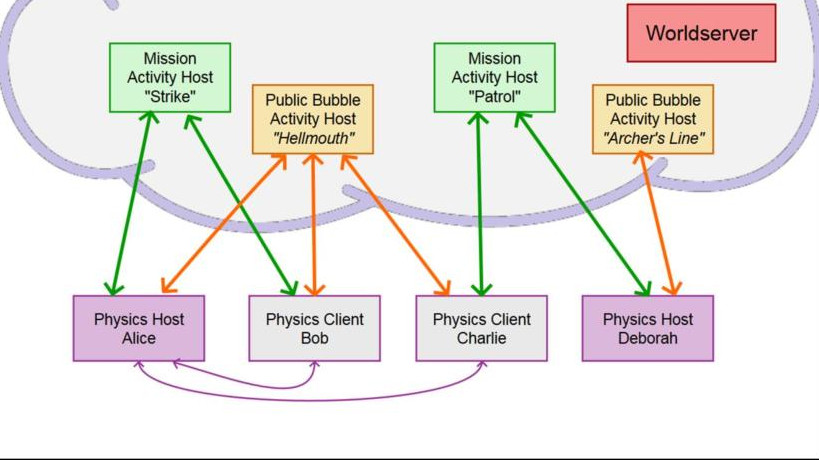
\includegraphics[width=0.5\textwidth]{Destiny2_networking}
  \caption{Example of how netcode is designed in Destiny 2. Image from the GDC talk: \mycite{truman2015destiny2}}
  \label{fig:destiny2netcode}
\end{figure}

\subsection{Issues with the peer to peer system}
The largest issues plaguing the games implemented with the peer to peer system all can be traced back to inconsistancies of state between the peers. This is inevetable when a delay is present in communication between parties. The paper \mycite{Carter2009} discusses some possible solutions that aim to mitigate or eliminate the idea of desynchronised game state. In general, during network communication, it can be sometimes be assumed that the connection is reliable however we can not assume that messages will arrive in the same order as they are sent.

The first idea that is suggested is called ``dead reckoning''. The paper \mycite{smed2002review} discusses this topic in detail. This is the idea of estimating what value is likely to be received from the server in the next packet by evaluating the previous values. In an example of an entity moving through a virtual environment at a constant speed in a constant direction and given that the position of this entity is being broadcasted from another entity, the game client can predict that if the previous packets have updated the position of this entity by the same amount every time, it can calculate the next value that will be received before the packet even arrives. This information can be used to interpolate the position of this entity between the packet that has just arrived and what poition it is expected to be in after the next packet arrives, thus giving the client a more smooth simulation. This also makes the smoothness of the simulation less reliant on network quality, though with low quality networking, the issue of ``rubber banding''\footnote{Rubber Banding is when a client sees an object in a simulation in a certain location but after a update of where this object should be arrives from an authority (server), this position is instantly updated to this new, correct position. From the client's point of view, this looks like the entity has teleported to the new location.} can become prevelent.

Another idea suggested is called ``local lag'' which involves the idea of puting incoming packets into a queue before they are used in the game. Using this method, if packets arrive out of order, they can be put in-order in the local buffer. In some game implementations, two actions performed in different order could result in a different outcome (for example rotating a character and moving them forwards). A potential downside that can arrise from using this method however, involves the fact that additional delay is incorporated to the process of sending information. This makes use of a system like this in games that require timely reactions potentially degrading for the players' experience. Local lag can be implemented in conjunction with dead reckoning for potentially better results.

Finally, an option called ``time warp'' can be utilised for synchronising game state. This technique is often used and well known in the field of Parallel and distributed Discrete Event Simulation (PDES). The paper \mycite{Jefferson1985} explains this topic in detail and ``Time Warm Mechanism'' is well explained. This mechanism listens and applies updates received from other peers when they arrive however, periodic ``snapshots'' of the entire game state are saved. If an inconsistancy is observed (for example if a straggler message is received from another peer), a ``rollback'' is applied to reset the simulation to a previous state, before the inconsistancy was observed. The system would also have to assume that any messages sent before the rollback was performed, were done so under inacurate assumptions. If this is the case, the peer can send a ``null-message'' which would inform the other peers of the inconsistancy and lead them to performing their own ``rollbacks''. This system can often cause ``network floods'' of ``null-messages''.

The system of ``local lag'' assumes that inconsistencies will always occur whereas ``time warp'' can often be concidered to be ``optimistic approaches'' because they allow each client to calculate their simulation state assuming no inconsistancies. Both implementations have uses in different scenarios.

\section{Other networking developement tools}
In this section, I will identify and investigate some tools that are available to developers for networked game developement as well as potential new technologies that could make a large imact on multiplayer online games.


\subsection{Google's Stadia and future networking options}
At the Game Developers Conference in March 2019, Google has announced a new Game Streaming platform. The talk outlined the plans that would allow developers to develop games for their Linux based platform that would run the game code on Google servers. Users of this service, would be able to play games by sending their inputs to the google servers. All game logic processing would then take place on the Google servers and the audio and video would be returned to the player. This service could potentially allow players to play games on devices with very little processing power, with settings that would normally require much more power.

A potential unexpected advantage of this system, could allow for networking possibilities that would be difficult to make work with current technologies. If a multiplayer game was developed for this system, it could allow for large scale virtual worlds with many players in the same instance as only one simulation would have to be processed for all the players. Each player's perspective would then be sent to them, this wouldn't be much different from how this system would function in a single player scenario.

The largest potential issue with a system like this could be the latency between the player sending an input to the server and then seeing this input reflected in the output. If this latency can be made neglegible through high speed internet connections and high processing power servers, it is possible that a system like this could work. If this latency can be minimised however, this system could prove to be a model that provides the best networking performance for large scale multiplayer experiences.


\newpage
\subsection{Networking options in Unity}
A game engine has been described as a core of controlling games by providing the main framework and common functions in the paper \mycite{xie2012research}. Unity is just one example of many different game engines that are avaliable to a developer, which all aim for the same unified goal but try to achieve it in different ways. Unity is a popular choice for projects ranging from small indie titles to large AAA productions and it is known for being relatively easy to use and prototype with. To investigate the options that are available in the market for online game developement, I have decided to investigate how networking functionality can be implemented in this game engine.

I have implemented a simple 2D game which allows the player fire a projectile, jump and move their character left and right. The goal with this project was to go through the process of transforming a simple, single player game to a simple multiplayer game through the use of different options available in Unity.

\subsubsection{UNET}
The first method of networking that I have decided to investigate was Unity's own UNET library. UNET uses the client hosted model that requires one client to act as a game server allowing others to connect to it. The joining clients need to know the IP address of the host in order to connect to them and the host can either join the game themselves or act purely as a server. The figures \ref{fig:unet_ui}, \ref{fig:main} and \ref{fig:in_game}, show screenshots of the default UI that is provided by the library as well as my game showing the main menu, client and server perspectives respectively. The tile-based pixel art used in the game has been found on the Unity Store under the name ``Sunny Land Forest'' and has been designed by Ansimuz.

Initially, the implementation of networking features proved to be very simple. A networking manager had to be added to the main scene and the networked scene had to be chosen. Spawn points, and the order that they should be used in, was easy to configure and the UI that allowed the user to connect and play was a simple addition too. Once two different player characters were spwaned in, there were some changes that had to be made to the movement scripts that involved specifying different behaviour whether the given character ``belongs'' to this player, or the other player. Checking if the character belonged to the player was as simple as comparing one boolean. This change can be seen in the change of colour of the character to blue if it is not the player controlled character in figure \ref{fig:in_game}.




\begin{figure}[p]
  \centering
  \subfloat[Main Menu UI]{
    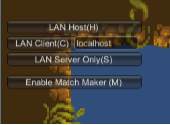
\includegraphics[width=0.3\linewidth]{UNET/Main_Menu_UI}
  }
  \qquad
  \subfloat[Host UI]{
    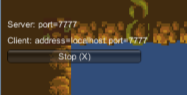
\includegraphics[width=0.3\textwidth]{UNET/Host_UI}
  }
  \qquad
  \subfloat[Client UI]{
    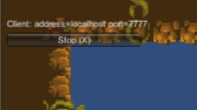
\includegraphics[width=0.3\linewidth]{UNET/Client_UI}
  }

  \caption{UNET default UI}
  \label{fig:unet_ui}
\end{figure}

\begin{figure}[p]
  \centering
  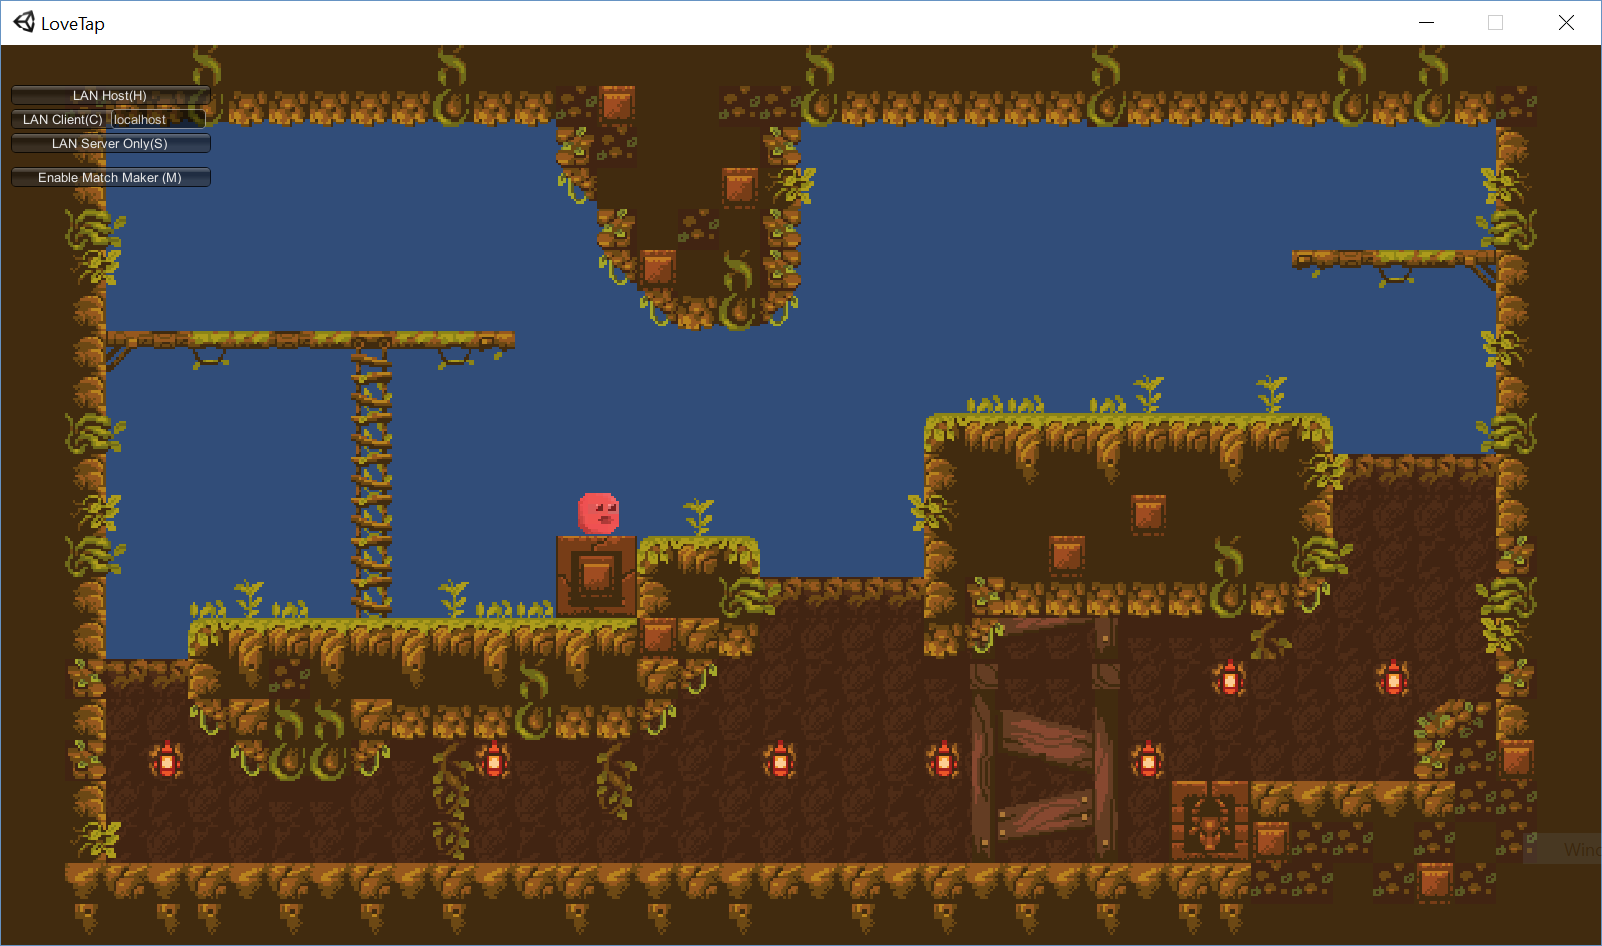
\includegraphics[width=\textwidth]{UNET/Main_Menu}
  \caption{Main Menu}
  \label{fig:main}
\end{figure}


\begin{figure}[p]
  \centering

  \subfloat[Host game screen]{
    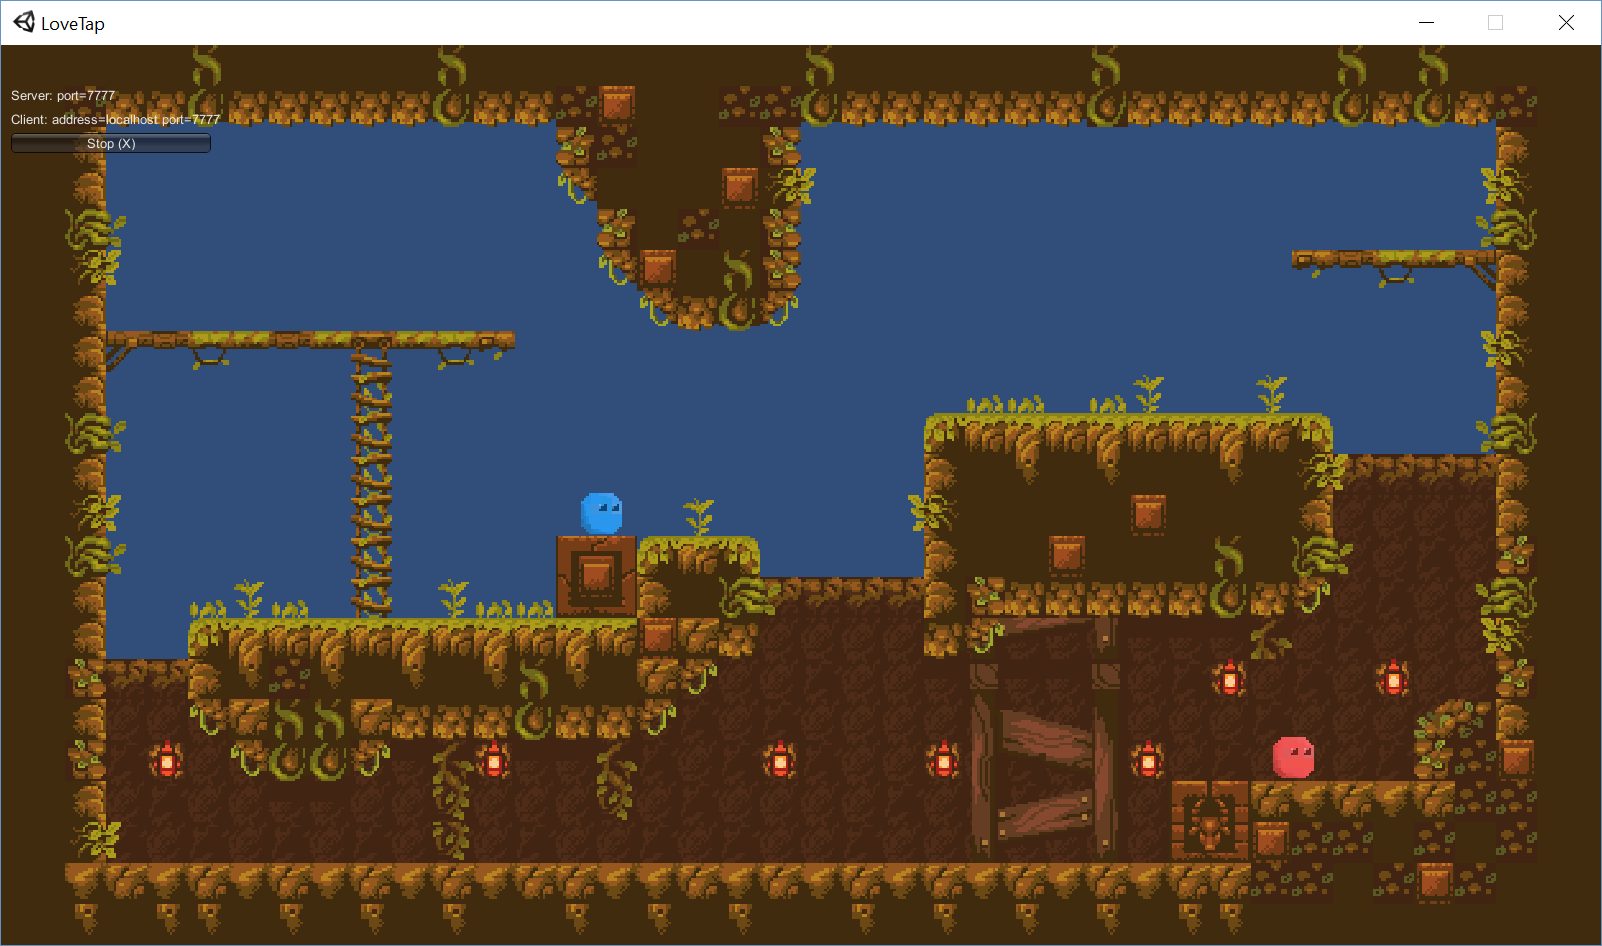
\includegraphics[width=0.45\textwidth]{UNET/Host}
  }
  \qquad
  \subfloat[Client game screen]{
    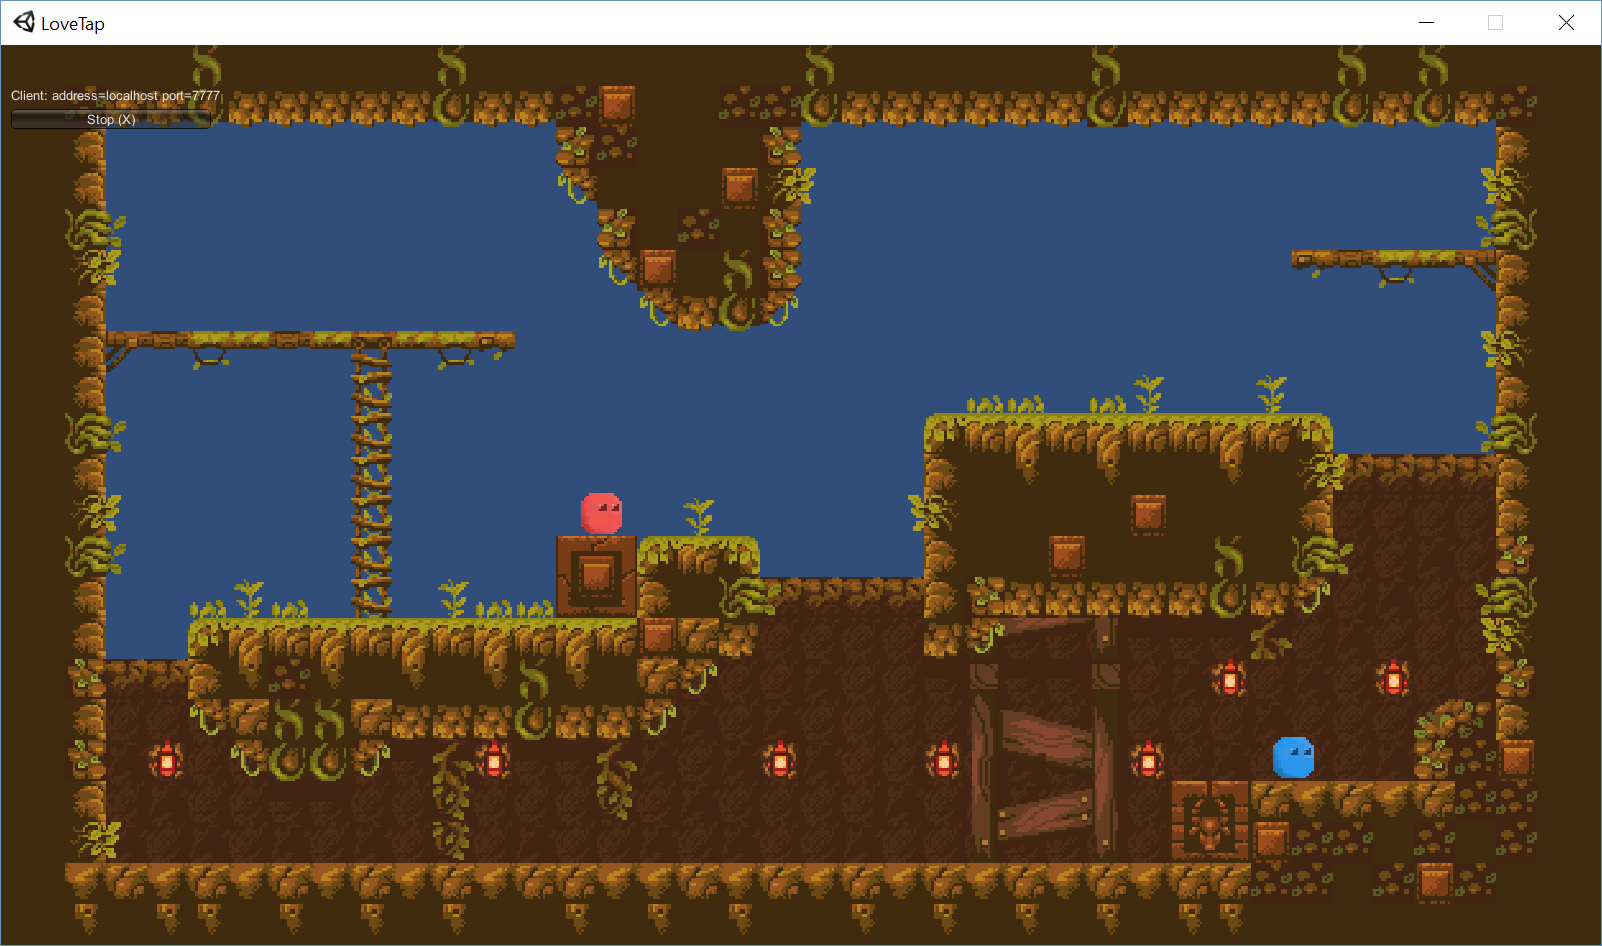
\includegraphics[width=0.45\linewidth]{UNET/Client}
  }

  \caption{Main game loop after connection is established}
  \label{fig:in_game}
\end{figure}

\newpage

\subsubsection{PUN (Photon Unity Network)}
PUN is an example of a 3rd party solution for networking in Unity.


\section{Related work summary}
TODO: what I am going to focus on and why and this leads nicely into chapter 3


\chapter{Design}

\section{Code Architecture}

Test for inline: \lstinline{test Hello;}

\section{Protocols}
During any connection that can be deployed between several processes on a machine or even different physical hardware in seperate geographical locaitons, many different protocols come into play.

\subsection{Protocols in Network Communications}
Firstly, in the network layer, most commonly the IP\footnote{IP: Internet Protocol} is employed however other options such as X.25 are also available but have more niche uses. These protocols are responsible for ``packaging'' the data to be sent between two different computers identified by their IP address. The packet from the sending machine, will travel through a network of routers that will eventually lead it to the machine with the IP address of the recieving machine.

Next comes the transport layer where either UDP\footnote{UDP: User Datagram Protocol} or TCP\footnote{TCP: Transfer Control Protocol}  can be chosen, both have different properties, advantages, disadvantages, useses and both are used in game networking. The UPD protocol is a simple, connectionless protocol which will simply send a packet from one IP address to another. Since each packet sent with UDP, can take a different route through the router network, there is no guarantee that the packets will be received in the same order as they were sent in. Due to many different reasons, packet loss can occur, meaning that it also cannot be guaranteed that every packet sent with UDP will arrive at the destination at all. Despite these dissadvantages and due to the simplicity of how this protocol was designed with it's connectionless nature, it inately has a major advantage in the speed that the packets can just be sent out and forgotten about. The TCP protocol, is built upon UDP to add some important features for reliable data sharing at a cost of speen and use in real-time applications. The most important property of TCP includes the assurance that if a packet is not received by a recipient, it is requested to be resent to guarantee that every pacet that is sent, is also recieved. This also means that the packets are aranged in the same order that they were sent meaning that we can be sure that not only data will arrive at the destination, but it will arrive just as we sent it. This implementation has many obvious benefits and in most scenarios, the delay of possibly re-sending a packet if it was not received is neglegible. In real-time applications however, this is likely to be an unnecessary waste of time and resources as even id a packet is dropped and and resent, by that time, new updated information is available so resending the dropped packet is useless when a packet with new information could be sent at that time instead. Simply, old information is quickly outdated and it's more important to send new information then old, non-useful information.

The next layer of protocols is the Operating System Iterface or library, that is called by applications needing to share data using the above protocols. With Windows, a library called ``WinSock'' is often used, however other options are also available such as enet, asio, RakNet... This is where a programmer would be able to configure which protocols to use (Like TCP or UDP, IP or X.25 amongst many other configurable options).


\subsection{Message Structure Startegies}

\subsubsection{Data Representation}
There are many different ways that the same data can be represented and each one is carefully designed to be the most appropriate for it's use. Consider the two figures below of common ways of goruping complex data in an ``easily readable'' format; XML in Figure \ref{fig:xml-example} and JSON in Figure \ref{fig:json-example}. These example have been adapted from the article \mycite{fiedler2016packets}.

\newpage
\begin{figure}[!ht]
\begin{lstlisting}[language=xml]
<world_update world_time="0.0">
  <object id="1" class="player">
    <property name="position" value="(0,0,0)"></property>
    <property name="orientation" value="(1,0,0,0)"></property>
    <property name="velocity" value="(10,0,0)"></property>
    <property name="health" value="100"></property>
    <property name="weapon" value="110"></property>
    ... 100s more properties per-object ...
 </object>
 <object id="110" class="weapon">
   <property type="semi-automatic"></property>
   <property ammo_in_clip="8"></property>
   <property round_in_chamber="true"></property>
 </object>
 ... 1000s more objects ...
</world_update>
\end{lstlisting}

\caption{An example of a representation of world data in the XML format}
\label{fig:xml-example}
\end{figure}

\begin{figure}[!ht]
\begin{lstlisting}[language=xml]
{
  "world_time": 0.0,
  "objects": {
    1: {
      "class": "player",
      "position": "(0,0,0)",
      "orientation": "(1,0,0,0)",
      "velocity": "(10,0,0)",
      "health": 100,
      "weapon": 110
    }
    110: {
      "class": "weapon",
      "type": "semi-automatic"
      "ammo_in_clip": 8,
      "round_in_chamber": 1
    }
    // etc...
  }
}
\end{lstlisting}

\caption{An example of a representation of world data in the JSON format}
\label{fig:json-example}
\end{figure}

\newpage


\subsubsection{Checking for Packet Loss in connection}
The packet information could contain a certain amount of bits that would be incremented with each simulation step\footnote{A simulation step refers to a state of values that represent the current state of a simulation. Each time the values are updated, is a new simulation step. This is often done and broadcasted several times a second in central server models.}. This counter value could loop round when a maximum value is reached as long as several simulation steps in a row have unique values. The receiver could evaluate this value when received, checking if a packet has been dropped since the last received update. Knowledge about the quality of the connection could be important information when determining how much of the simulation has to be estimated between the received updates and could also be vital information to the player when in a game demanding split-second reaction time allowing them to change their strategy with the knowledge that they may be at a dissadvantage against other players.



\newpage

%fig:client-protocol
\begin{figure}[h]

  \centering
  \begin{sequencediagram}
    \newthread{client}{Client}{}
    \newinst{server-lsn}{Server Listener}{}
    \newinst{key-lsn}{Keyboard Listener}{}
    \newthread{server}{Server}{}

    \begin{sdblock}{Connection}{}

      \begin{call}{server}{openToClientConnection()}{server}{\textit{Once all clients connect...}}
        \postlevel
        \postlevel
        \postlevel
        \postlevel
      \end{call}

      \prelevel \prelevel \prelevel
      \prelevel \prelevel
      \mess{client}{JR}{server}
      \begin{call}{client}{listenForServerMsg()}{client}{}
        \mess{server}{JA<ID>}{client}
      \end{call}


      \begin{call}{client}{listenForServerMsg()}{client}{}
        \mess{server}{DE< <ID><VAL> ... >}{client}
      \end{call}
    \end{sdblock}

    \begin{sdblock}{Update Loop}{}

      \begin{call}{server}{startUpdateLoop()}{server}{\textit{simulation finished}}
        \postlevel \postlevel \postlevel
        \postlevel \postlevel \postlevel
      \end{call}
      \prelevel \prelevel \prelevel
      \prelevel \prelevel \prelevel


      \begin{call}{client}{startServerListen()}{server-lsn}{\textit{loop}}
        \mess{server}{CS< <ID><VAL> ... >}{server-lsn}
        \postlevel \postlevel \postlevel
      \end{call}

      \prelevel \prelevel \prelevel
      \begin{call}{client}{startKeyboardListen()}{key-lsn}{}
        \mess{key-lsn}{UP<VAL>}{server}
      \end{call}

    \end{sdblock}
  \end{sequencediagram}

  \caption{Graph showing the protocol of joining a session hosted on the server as well as sending and receiving updates.}
  \label{fig:client-protocol}
\end{figure}


\subsection{Potential issues with the Client Hosted protocol}
The protocol for establishing a connection and transfering of data can be found in Figure \ref{fig:client-protocol}. There are many potential flaws with this approach.
\subsubsection{Packet Loss}
Time outs in place in case response lost...
resend....
Resend request if no response....


\subsubsection{Security}
anyone could send update by spoofing ip


\pagebreak
\section{Message Codes}

%table:message-codes
\begin{table}[t]
  \centering
  \begin{tabular}{ l l p{0.3\textwidth} l }
    \toprule
    Message Type & Message Code & Description & Example Payload \\
    \midrule
    Join Request &
      \lstinline[]$JR$ &
      Allows a client to send a join request to the server. &
      \lstinline[]$JR$ \\
    \addlinespace[10pt]
    Join Acknowledgement &
      \lstinline[]$JA$ &
      Allows the server to confirm that the client's information has been saved. Is followed by 1 byte indicating the client's ID &
      \lstinline[]$JA1$ \\
    \addlinespace[10pt]
    Ping Request &
      \lstinline[]$PQ$ &
      Message instructing the recipiant to reply with \lstinline[]$PS$. Can be used to time the delay in this connection.&
      \lstinline[]$PQ$ \\
    \addlinespace[10pt]
    Ping Response &
      \lstinline[]$RS$ &
      This should be sent whenever a \lstinline[]$PQ$ message is received. &
      \lstinline[]$RS$ \\
    \addlinespace[10pt]
    Update &
      \lstinline[]$UP$ &
      Used by a client to update it's value on the server. Is followed by 1 byte representing the new value. &
      \lstinline[]$UP9$ \\
    \addlinespace[10pt]
    Define &
      \lstinline[]$DF$ &
      Used by the server to define the initial values for each of the clients connected to this instance. It is followed by a non-zero, even amount of bytes representing the client ID and it's value pair. &
      \lstinline[]$DF1020304050$ \\
    \addlinespace[10pt]
    Current State &
      \lstinline[]$CS$ &
      Used by the server to broadcast it's real state to all clients. When this is received, clients are expected to update their local state to this. It is followed by a non-zero, even amount of bytes representing the client ID and it's value pair. &
      \lstinline[]$CS1927344157$ \\

    \bottomrule
  \end{tabular}
  \caption{Table showing the message codes for distinguishing messages from each other and how each one is to be used}
  \label{table:message-codes}
\end{table}


\pagebreak

\appendix
\chapter{Networking Model Attributes}\label{app:attributes}

\section{Central Server Model}
\begin{figure}[!h]
  \begin{tabular}{ c p{0.94\textwidth} }
    \faCheckCircle & Hardware is likely to be powerful enough to handle the stress of many simulations running simultaneously. \\
    \faCheckCircle & High bandwidth connection is likely to be used. Minimises the chance of high latency and network issues. \\
    \faCheckCircle & Ping to the server is likely to be similar for all players making the game more fair.  \\
    \faCheckCircle & No client can see the address of any other client. \\
    \faCheckCircle & The developer has a lot of control over what is allowed within the game. This allows for anti-cheating systems that are hard to bypass. \\
    \  & \  \\
    \faTimesCircle & Expensive to rent out, or buy and maintain, server space. Letting players rent out servers makes the game more expensive for them. \\
    \faTimesCircle & Many servers have to be spread out evenly throughout the world to allow for low latency connections.  \\
    \faTimesCircle & People living in remote locations may not have low latency access to official servers.
  \end{tabular}
  \caption{The attributes of the central server model}
  \label{fig:cs_attributes}
\end{figure}

\newpage

\section{Client Hosted Model}
\begin{figure}[!h]
  \begin{tabular}{ c p{0.94\textwidth} }
    \faCheckCircle & There are no additional costs to the publisher/developer when releasing the game. \\
    \faCheckCircle & Players in remote locations can play together with low latency. \\
    \faCheckCircle & The codebase is relatively easily transferable to a central server model if the need arises. \\
    \  & \  \\
    \faTimesCircle & The host player has negligible ping to the server. This could be a large advantage.  \\
    \faTimesCircle & The host player is likely to use a consumer grade connection increasing the risk of packet loss and high latency \\
    \faTimesCircle & The host player could be using WiFi to host the game which could significantly increase the chance of packet loss. \\
    \faTimesCircle & The host's hardware may not be powerful enough to calculate each simulation step within an acceptable tick rate. \\
    \faTimesCircle & If the host player is disconnected mid-game, a host migration will have to take place pausing the game for a few seconds or causing the game to finish unexpectedly. \\
    \faTimesCircle & The host player can see the IP address of each other player that they are playing with. \\
    \faTimesCircle & Cheating could be easy if the host player sends malicious packets to the clients pretending to be the game server.

  \end{tabular}
  \caption{The attributes of the client hosted model}
  \label{fig:ch_attributes}
\end{figure}

\newpage

\section{Peer to Peer model}
\begin{figure}[!h]
  \begin{tabular}{ c p{0.94\textwidth} }
    \faCheckCircle & There are no additional costs to the publisher/developer when releasing the game. \\
    \faCheckCircle & Players in remote locations can play together with low latency. \\
    \faCheckCircle & There is no concept of host advantage, like what is present with the client hosted model. \\
    \faCheckCircle & Host migrations are not a large problem since everyone has the full simulation state. \\
    \  & \  \\
    \faMinusCircle & Each client communicates directly with other clients making their connection as efficient as possible in theory. \\
    \faMinusCircle & Even though a central ``authority'' is not needed, one of the peers often has to act as a session host to handle invitations and handshakes. \\
    \faMinusCircle & Every client runs it's own simulation and is tasked with keeping it updated with everyone else's. \\
    \  & \  \\
    \faTimesCircle & The lack of a central authority (such as a game server) makes cheat prevention difficult. \\
    \faTimesCircle & Each player in an instance, can see the IP address of every other player they are playing with. \\
    \faTimesCircle & Interacting with two different peers with different latencies, will feel inconsistant for the player.  \\
    \faTimesCircle & Very high bandwidth usage compared to other models. \\
    \faTimesCircle & The amount of update messages that need to be sent, increases as the number of players grows. \\
    \faTimesCircle & A player with a poor internet connection or underpowered hardware, will make the game feel less responsive to other players. \\
   \end{tabular}
  \caption{The attributes of the peer to peer model}
    \label{fig:p2p_attributes}
\end{figure}


\chapter{Jitter Variance table}

\begin{table}[!h]
  \centering
  \begin{tabular}{ l r r r }
    \toprule
    Delay between messages (ms) & WiFi & Ethernet & Localhost \\
    \midrule

     8     & 3.67E-06       & 3.74E-06 & 3.46E-06 \\
     64    & 8.81E-07       & 5.67E-07 & 4.61E-07 \\
     125   & 1.54E-06       & 8.68E-07 & 8.16E-07 \\
     250   & 1.46E-06       & 9.19E-07 & 7.72E-07 \\
     500   & 3.62E-05       & 1.63E-07 & 8.40E-08 \\
     1000  & 0.009563789805 & 3.18E-07 & 1.84E-07 \\

    \bottomrule
  \end{tabular}
  \caption{Table showing the variance values of the jitter seen in test result}
  \label{table:var_table}
\end{table}


\chapter{Developement Issues}
\begin{figure}[!h]
  \centering
  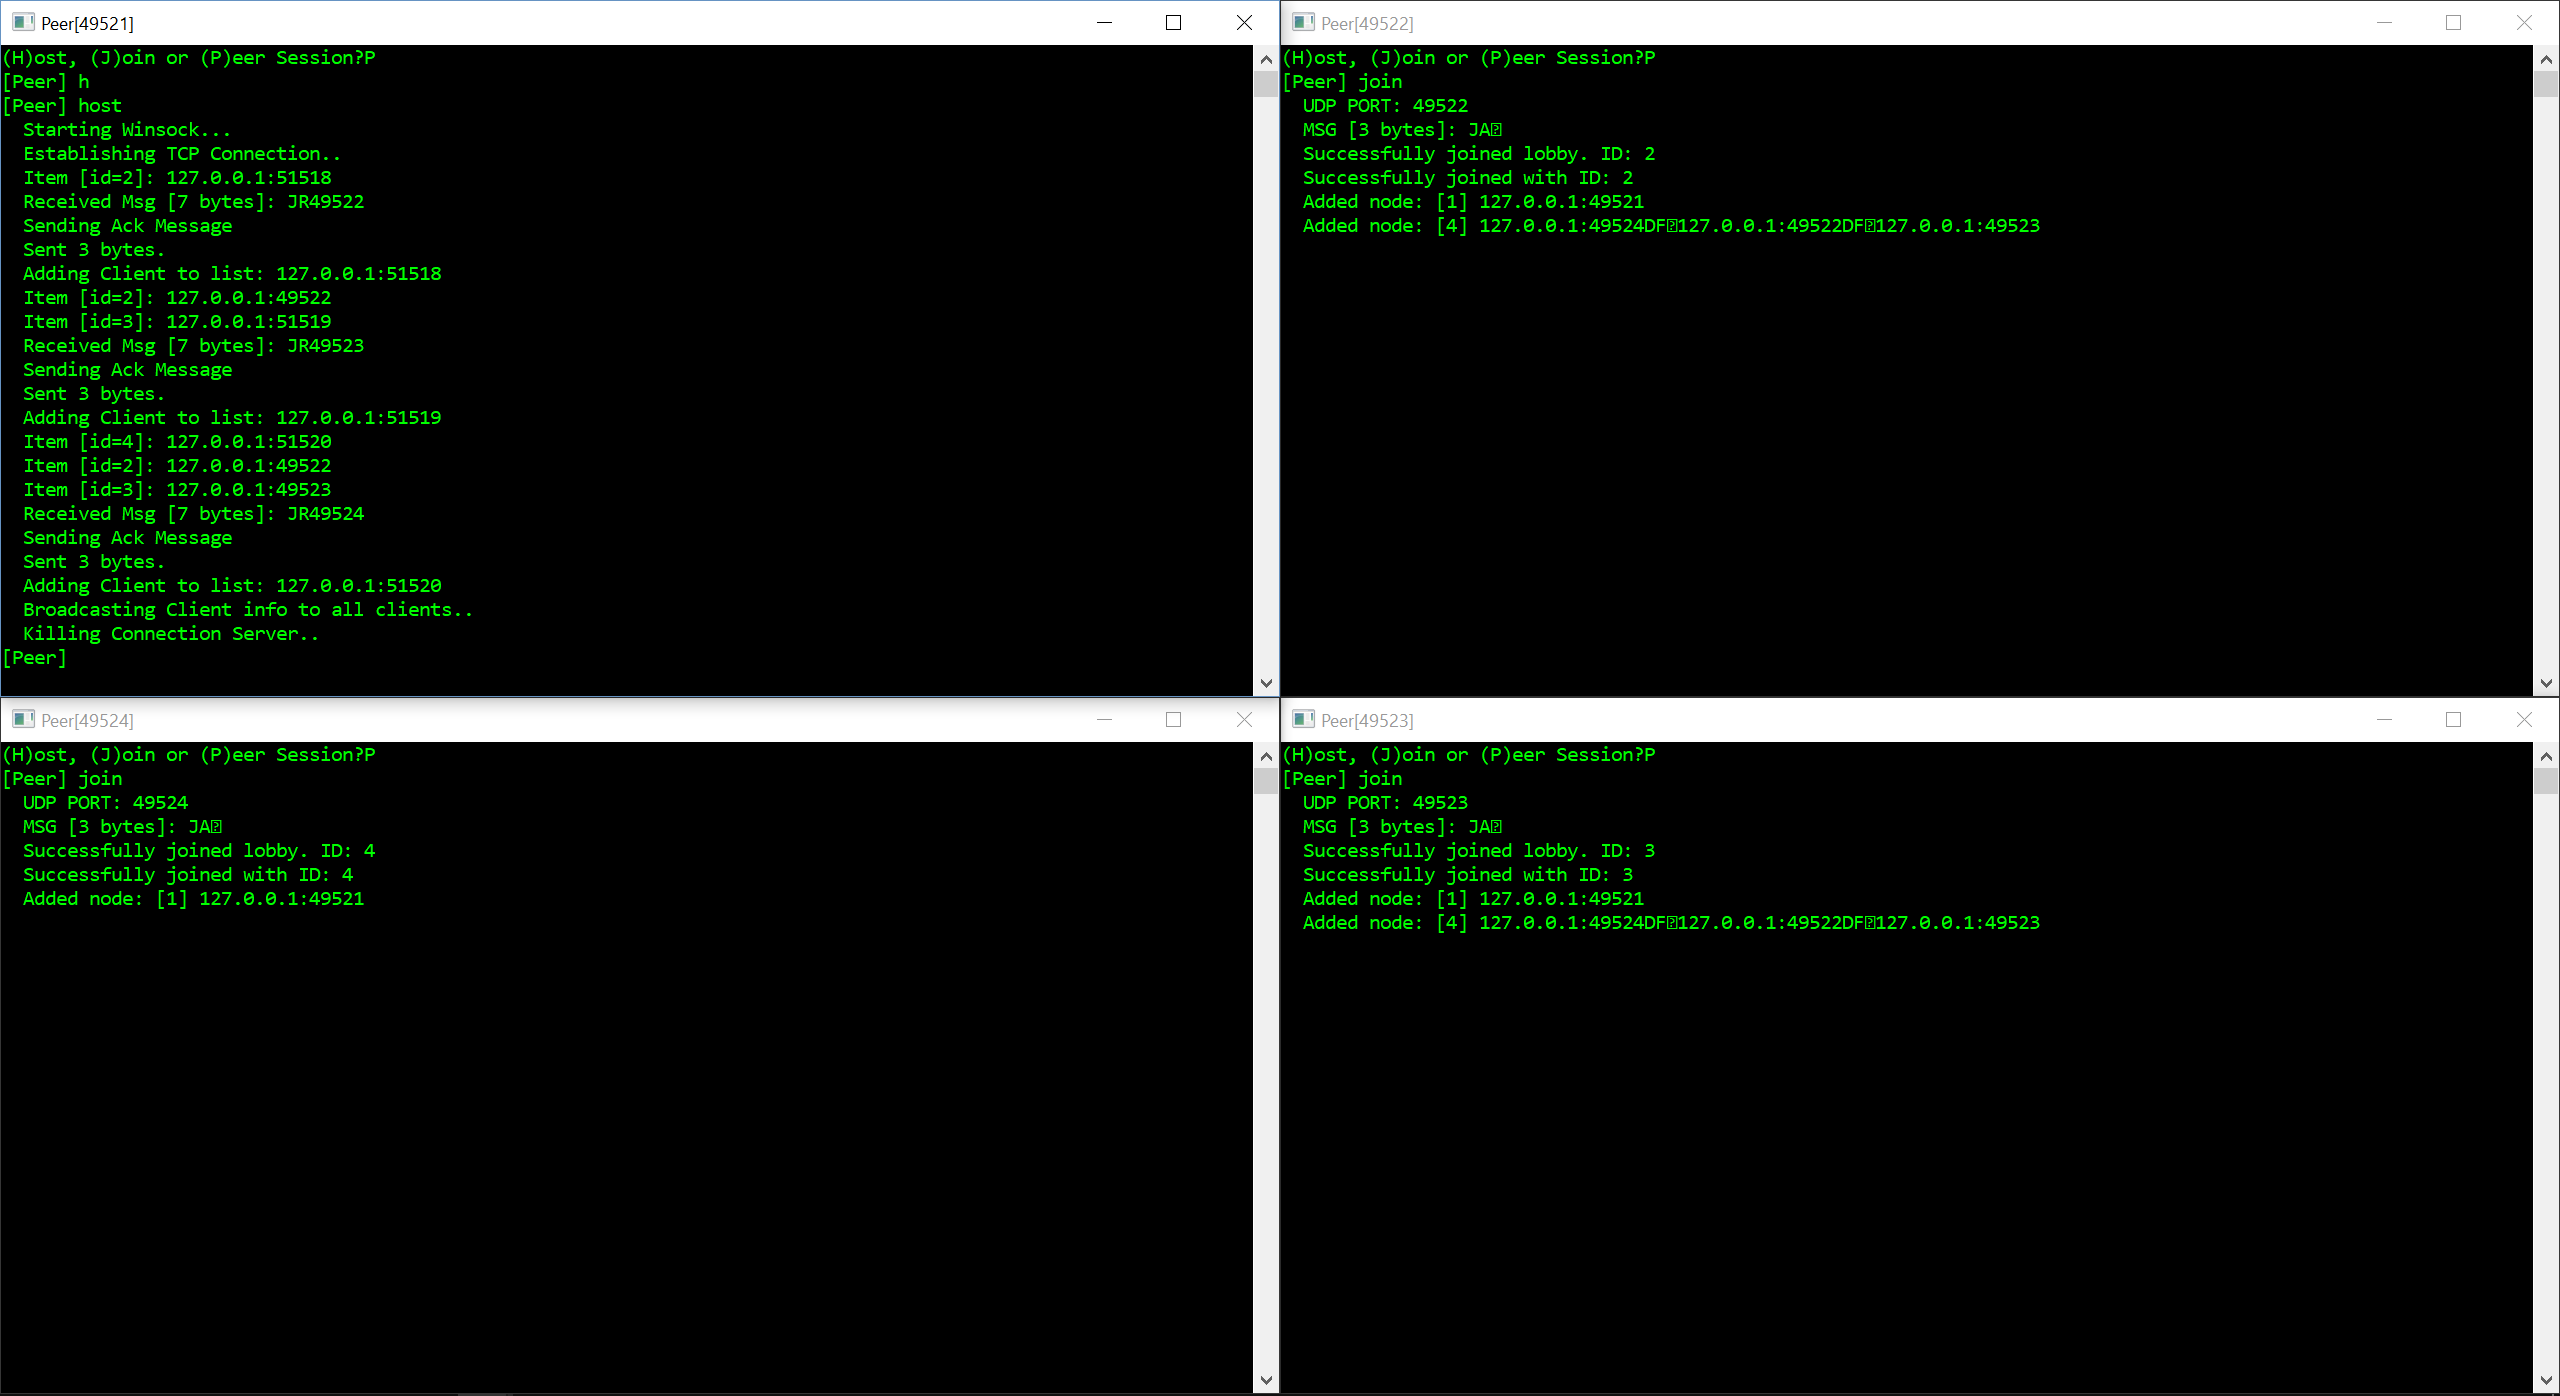
\includegraphics[width=\textwidth]{GNAT/sending_too_fast.png}
  \caption{Messages being broadcast with no delay}
  \label{fig:broadcast_too_fast}
\end{figure}

\begin{figure}[!h]
  \centering
  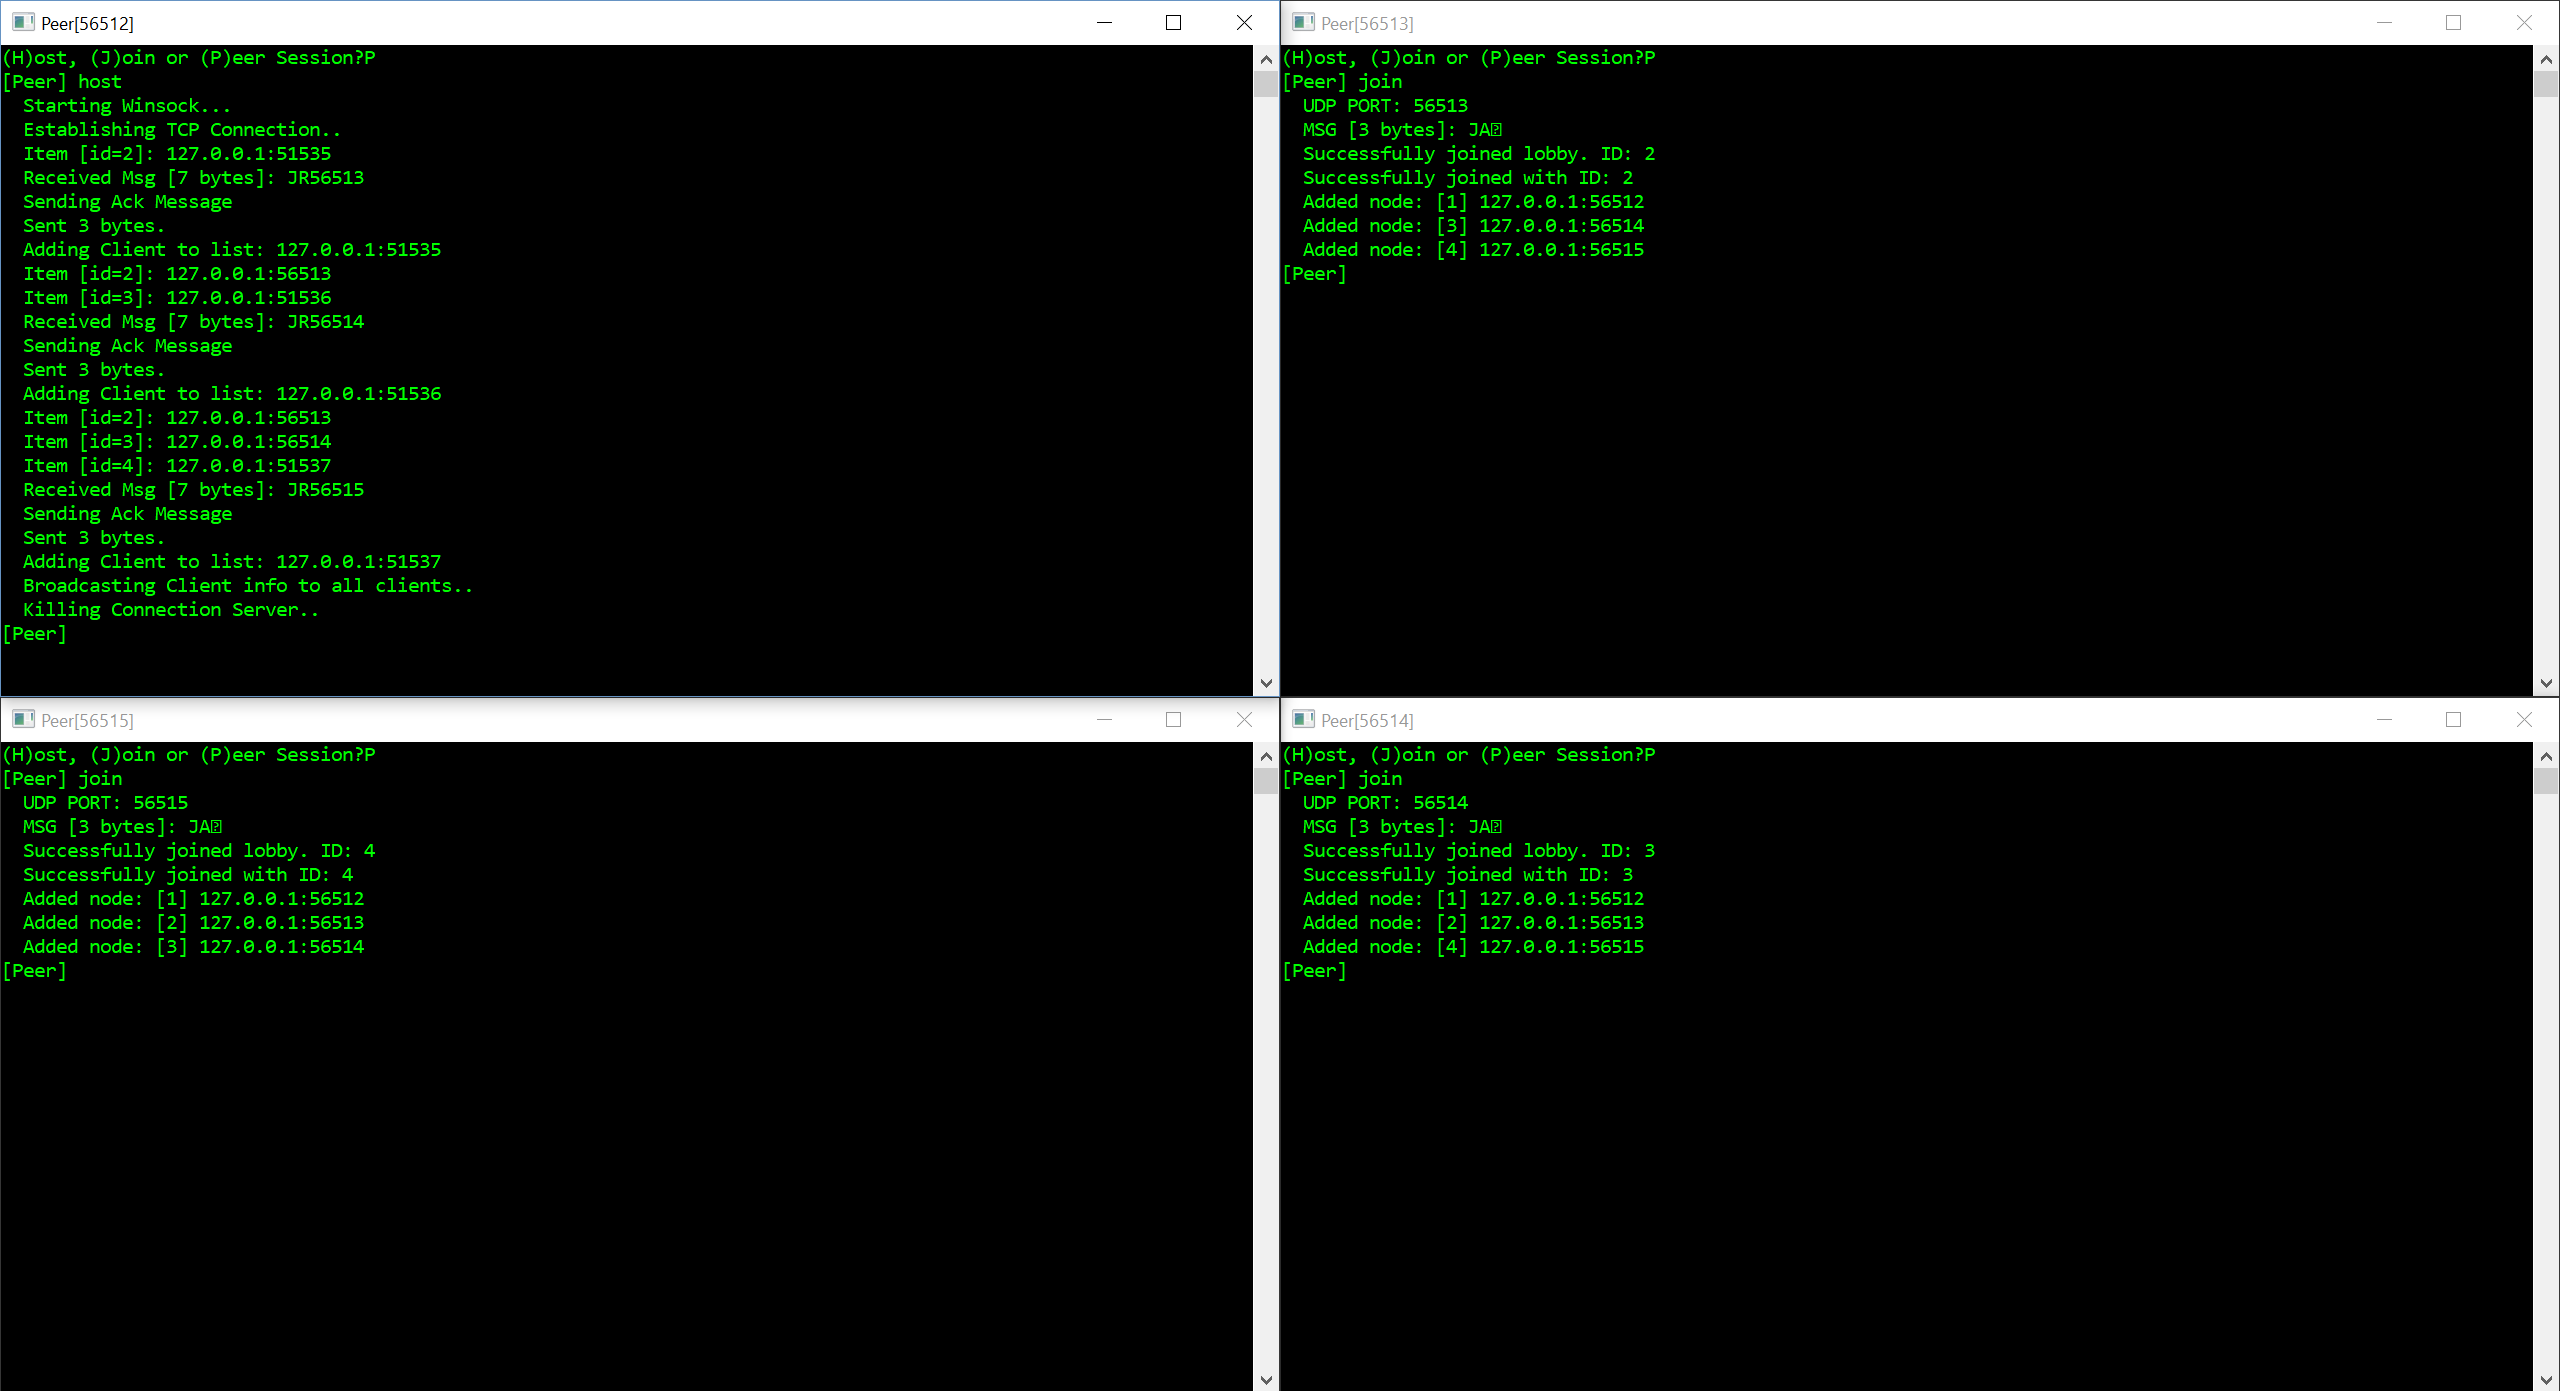
\includegraphics[width=\textwidth]{GNAT/sending_with_delay.png}
  \caption{Messages being broadcast with delay}
  \label{fig:broadcast_with_delay}
\end{figure}

\chapter{GNAT Code Snippets}

\section{Pre-compiled Headers}
When developing a project that uses code that will not change, such as the std library and winsock, it is inefficient to compile the code for these libraries every time the project code is compiled. To greatly improve compile times, precompiled headers are used.

\textbf{pch.h}
\begin{lstlisting}
// General
#include <string>
#include <iostream>
#include <thread>

// Data Structures
#include <map>
#include <vector>

// WinSock
#include <winsock2.h>
#include <Ws2tcpip.h>
#include <windows.h>

#pragma comment (lib, "ws2_32.lib")

// Custom
#include "log.h"
\end{lstlisting}

\textbf{pch.cpp}
\begin{lstlisting}
#include "pch.h"
\end{lstlisting}


\section{Logging library wrapper}
For the logging library, a 3rd party project was used called spdlog. The wrapper is used to use this library in predefined ways.


\textbf{Log.h}
\begin{lstlisting}
#pragma once
#include <memory>
#include <spdlog/spdlog.h>

namespace GNAT {
	class GNAT_Log {
	public:
		static void init();
		static void init_client();
		static void init_server();
		static void init_peer();
		static void init_connection();

		inline static std::shared_ptr<spdlog::logger>& getConnectionLogger() { return connection_logger; }
		inline static std::shared_ptr<spdlog::logger>& getServerLogger() { return server_logger; }
		inline static std::shared_ptr<spdlog::logger>& getPeerLogger() { return peer_logger; }
		inline static std::shared_ptr<spdlog::logger>& getClientLogger() { return client_logger; }

	private:
		const static int LOG_FILE_SIZE_IN_MB = 5;
		const static int ROTATING_FILE_COUNT = 3;

		static std::shared_ptr<spdlog::logger> connection_logger;
		static std::shared_ptr<spdlog::logger> server_logger;
		static std::shared_ptr<spdlog::logger> peer_logger;
		static std::shared_ptr<spdlog::logger> client_logger;
	};
}

// Loging Macros
#define CONNECT_LOG_FATAL(...) GNAT::GNAT_Log::getConnectionLogger()->fatal(__VA_ARGS__); std::cout << "  " << __VA_ARGS__ << std::endl
#define CONNECT_LOG_ERROR(...) GNAT::GNAT_Log::getConnectionLogger()->error(__VA_ARGS__); std::cout << "  " << __VA_ARGS__ << std::endl
#define CONNECT_LOG_WARN(...) GNAT::GNAT_Log::getConnectionLogger()->warn(__VA_ARGS__);	 std::cout << "  " << __VA_ARGS__ << std::endl
#define CONNECT_LOG_INFO(...) GNAT::GNAT_Log::getConnectionLogger()->info(__VA_ARGS__);	 std::cout << "  " << __VA_ARGS__ << std::endl
#define CONNECT_LOG_TRACE(...) GNAT::GNAT_Log::getConnectionLogger()->trace(__VA_ARGS__); std::cout << "  " << __VA_ARGS__ << std::endl

#define SERVER_LOG_FATAL(...) GNAT::GNAT_Log::getServerLogger()->fatal(__VA_ARGS__); std::cout << "  " << __VA_ARGS__ << std::endl
#define SERVER_LOG_ERROR(...) GNAT::GNAT_Log::getServerLogger()->error(__VA_ARGS__); std::cout << "  " << __VA_ARGS__ << std::endl
#define SERVER_LOG_WARN(...) GNAT::GNAT_Log::getServerLogger()->warn(__VA_ARGS__);	 std::cout << "  " << __VA_ARGS__ << std::endl
#define SERVER_LOG_INFO(...) GNAT::GNAT_Log::getServerLogger()->info(__VA_ARGS__);	 std::cout << "  " << __VA_ARGS__ << std::endl
#define SERVER_LOG_TRACE(...) GNAT::GNAT_Log::getServerLogger()->trace(__VA_ARGS__); std::cout << "  " << __VA_ARGS__ << std::endl

#define PEER_LOG_FATAL(...) GNAT::GNAT_Log::getPeerLogger()->fatal(__VA_ARGS__);	 std::cout << "  " << __VA_ARGS__ << std::endl
#define PEER_LOG_ERROR(...) GNAT::GNAT_Log::getPeerLogger()->error(__VA_ARGS__);	 std::cout << "  " << __VA_ARGS__ << std::endl
#define PEER_LOG_WARN(...) GNAT::GNAT_Log::getPeerLogger()->warn(__VA_ARGS__);		 std::cout << "  " << __VA_ARGS__ << std::endl
#define PEER_LOG_INFO(...) GNAT::GNAT_Log::getPeerLogger()->info(__VA_ARGS__);		 std::cout << "  " << __VA_ARGS__ << std::endl
#define PEER_LOG_TRACE(...) GNAT::GNAT_Log::getPeerLogger()->trace(__VA_ARGS__);	 std::cout << "  " << __VA_ARGS__ << std::endl

#define CLIENT_LOG_FATAL(...) GNAT::GNAT_Log::getClientLogger()->fatal(__VA_ARGS__); std::cout << "  " << __VA_ARGS__ << std::endl
#define CLIENT_LOG_ERROR(...) GNAT::GNAT_Log::getClientLogger()->error(__VA_ARGS__); std::cout << "  " << __VA_ARGS__ << std::endl
#define CLIENT_LOG_WARN(...) GNAT::GNAT_Log::getClientLogger()->warn(__VA_ARGS__);	 std::cout << "  " << __VA_ARGS__ << std::endl
#define CLIENT_LOG_INFO(...) GNAT::GNAT_Log::getClientLogger()->info(__VA_ARGS__);	 std::cout << "  " << __VA_ARGS__ << std::endl
#define CLIENT_LOG_TRACE(...) GNAT::GNAT_Log::getClientLogger()->trace(__VA_ARGS__); std::cout << "  " << __VA_ARGS__ << std::endl
\end{lstlisting}

\textbf{Log.cpp}

\begin{lstlisting}
#include "pch.h"
#include "log.h"
#include <spdlog/sinks/rotating_file_sink.h>
#include <ctime>

namespace GNAT {
	std::shared_ptr<spdlog::logger> GNAT_Log::connection_logger;
	std::shared_ptr<spdlog::logger> GNAT_Log::server_logger;
	std::shared_ptr<spdlog::logger> GNAT_Log::peer_logger;
	std::shared_ptr<spdlog::logger> GNAT_Log::client_logger;

	void GNAT_Log::init() {
		spdlog::set_pattern("%^[%T] %n: %v%$");

		try
		{
			peer_logger = spdlog::rotating_logger_mt("CONN", "Logs\\CONN-" + std::to_string(std::time(0)) + ".log", 1024 * 1024 * LOG_FILE_SIZE_IN_MB, ROTATING_FILE_COUNT);
			server_logger = spdlog::rotating_logger_mt("SERV", "Logs\\SERV-" + std::to_string(std::time(0)) + ".log", 1024 * 1024 * LOG_FILE_SIZE_IN_MB, ROTATING_FILE_COUNT);
			peer_logger = spdlog::rotating_logger_mt("PEER", "Logs\\PEER-" + std::to_string(std::time(0)) + ".log", 1024 * 1024 * LOG_FILE_SIZE_IN_MB, ROTATING_FILE_COUNT);
			client_logger = spdlog::rotating_logger_mt("CLNT", "Logs\\CLNT-" + std::to_string(std::time(0)) + ".log", 1024 * 1024 * LOG_FILE_SIZE_IN_MB, ROTATING_FILE_COUNT);
		}
		catch (const spdlog::spdlog_ex& ex)
		{
			std::cout << "Log initialization failed: " << ex.what() << std::endl;
		}
	}

	void GNAT_Log::init_client() {
		spdlog::set_pattern("%^[%T] %n: %v%$");

		try
		{
			client_logger = spdlog::rotating_logger_mt("CLNT", "Logs\\CLNT-" + std::to_string(std::time(0)) + ".log", 1024 * 1024 * LOG_FILE_SIZE_IN_MB, ROTATING_FILE_COUNT);
		}
		catch (const spdlog::spdlog_ex& ex)
		{
			std::cout << "Log initialization failed: " << ex.what() << std::endl;
		}
	}

	void GNAT_Log::init_server() {
		spdlog::set_pattern("%^[%T] %n: %v%$");

		try
		{
			server_logger = spdlog::rotating_logger_mt("SERV", "Logs\\SERV-" + std::to_string(std::time(0)) + ".log", 1024 * 1024 * LOG_FILE_SIZE_IN_MB, ROTATING_FILE_COUNT);
		}
		catch (const spdlog::spdlog_ex& ex)
		{
			std::cout << "Log initialization failed: " << ex.what() << std::endl;
		}
	}

	void GNAT_Log::init_peer() {
		spdlog::set_pattern("%^[%T] %n: %v%$");

		try
		{
			peer_logger = spdlog::rotating_logger_mt("PEER", "Logs\\PEER-" + std::to_string(std::time(0)) + ".log", 1024 * 1024 * LOG_FILE_SIZE_IN_MB, ROTATING_FILE_COUNT);
		}
		catch (const spdlog::spdlog_ex& ex)
		{
			std::cout << "Log initialization failed: " << ex.what() << std::endl;
		}
	}

	void GNAT_Log::init_connection() {
		spdlog::set_pattern("%^[%T] %n: %v%$");

		try
		{
			connection_logger = spdlog::rotating_logger_mt("CONN", "Logs\\CONN-" + std::to_string(std::time(0)) + ".log", 1024 * 1024 * LOG_FILE_SIZE_IN_MB, ROTATING_FILE_COUNT);
		}
		catch (const spdlog::spdlog_ex& ex)
		{
			std::cout << "Log initialization failed: " << ex.what() << std::endl;
		}
	}
}
\end{lstlisting}

\end{document}
